\subsubsection{Buffer}
Le funzioni \emph{rdt\_send} e \emph{rdt\_recv} fungono da regolatori del flusso
di dati dal livello applicativo puro a quello di trasporto virtuale e 
viceversa.\\
Queste funzioni comunicano con i thread di invio e ricezione tramite 
dei buffer condivisi secondo uno schema del tipo produttore-consumatore, in 
modo tale che i dati effettuino il passaggio di livello solo quando c'è spazio
disponibile sui buffer.
%
\begin{figure}[!h]
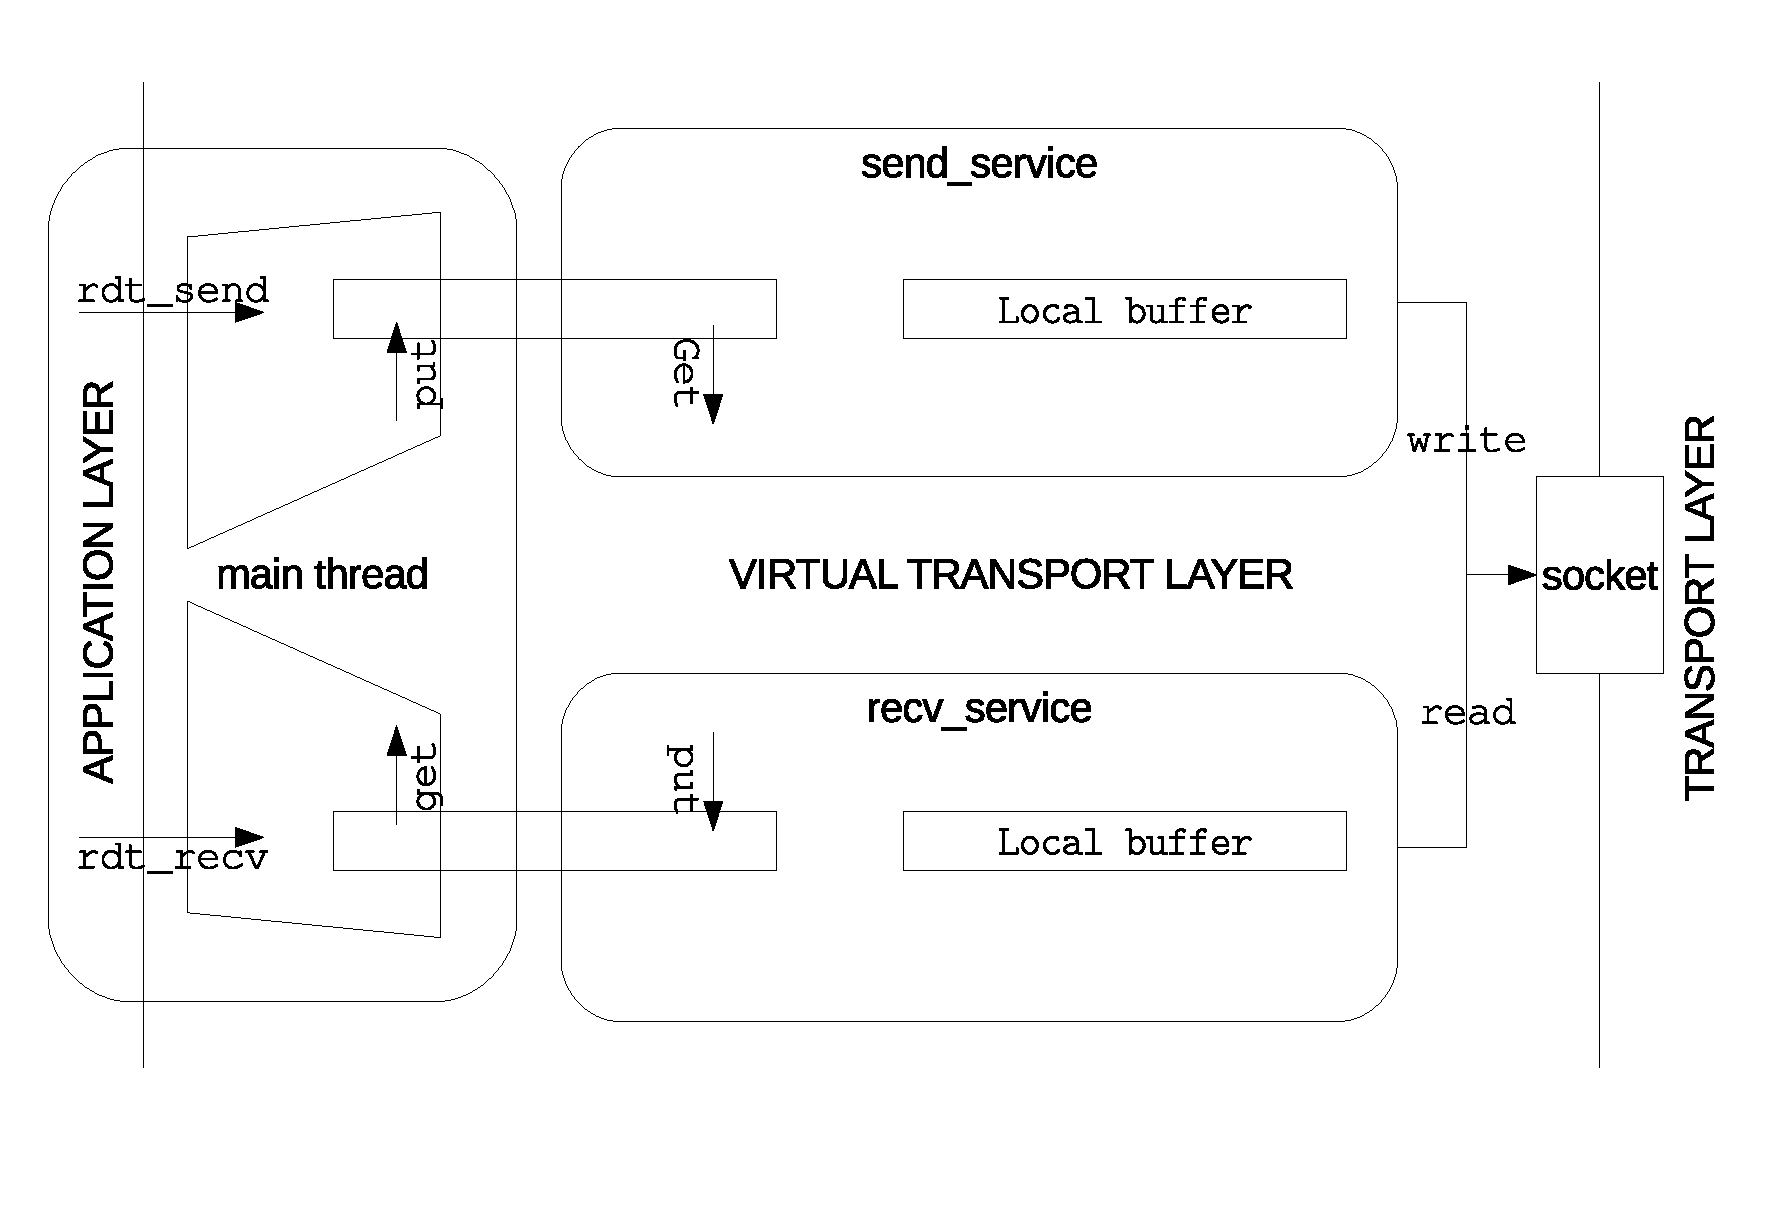
\includegraphics[scale=0.35]{images/structure_1}
\caption{Struttura generale del livello di trasporto virtuale}
\end{figure}
%
Come già detto, le unità di base con cui l'algoritmo ha a che fare sono
i segmenti che contengono i dati applicativi. Poiché tali segmenti sono
soggetti a ritrasmissioni, è necessario che vengano ``immagazzinati'' da 
qualche parte, inoltre, per quanto riguarda il lato destinatario, vanno
consegnati al livello applicativo in ordine, per queste ragioni, sia il 
servizio di invio che il servizio di ricezione sono dotati di buffer locali.\\
Tali buffer sono implementati tramite array di dimensione fissa e hanno una
capacità pari a MAXSEQNUM slot, in modo tale da far
corrispondere gli indici ai numeri di sequenza dei segmenti e 
garantirne un accesso immediato ($\mathcal{O}(1)$). Inoltre i buffer vengono
trattati come circolari, così da emulare naturalmente il riciclo dei numeri 
di sequenza.\\
Mentre il buffer del \emph{recv\_service} è implementato tramite un'array di 
strutture \emph{segment}, quello del \emph{send\_service} è un'array di 
strutture \emph{packet}, ovvero contenitori di segmenti e informazioni ad essi
relative necessarie al funzionamento del timeout, come istante di invio, quello
di scadenza ed un booleano che indica se il pacchetto è stato ritrasmesso.
%
\begin{lstlisting}[title=transport.h]
struct packet {
	struct segment sgt;
	struct timespec sendtime;
	struct timespec exptime;
	bool rtx;
};
\end{lstlisting}
